\documentclass[tikz,border=6pt]{standalone}
\usetikzlibrary{arrows.meta,positioning,fit}
\begin{document}
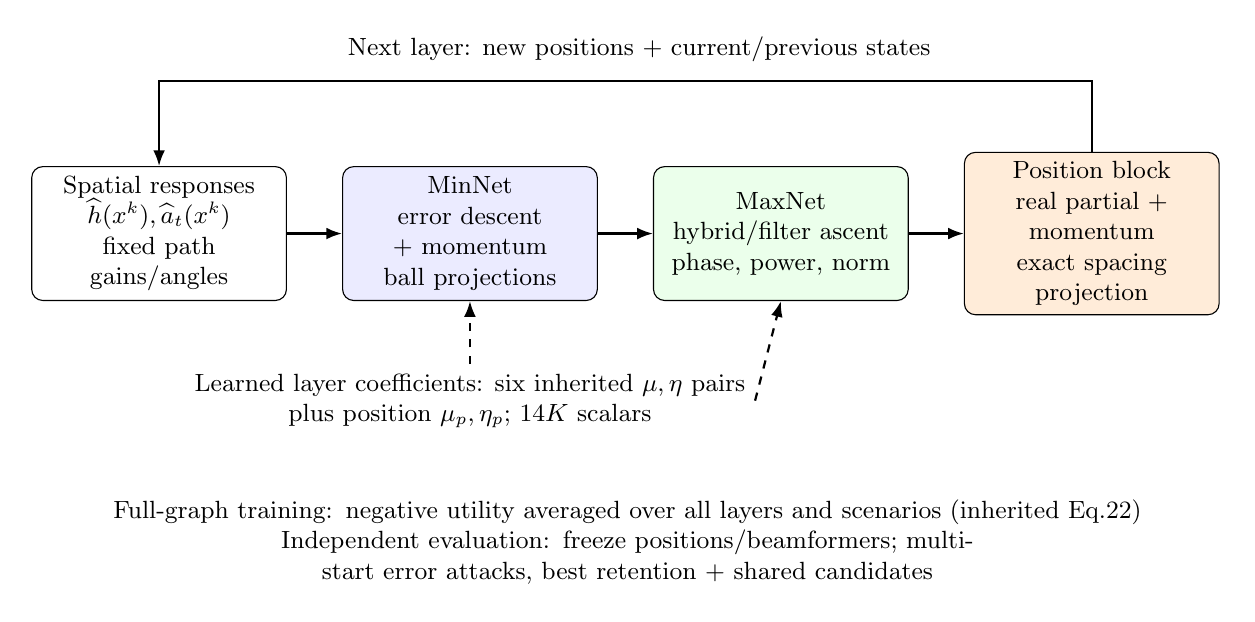
\begin{tikzpicture}[font=\small,block/.style={draw,rounded corners,align=center,text width=30mm,minimum height=17mm},arr/.style={-{Latex[length=2mm]},thick}]
\node[block] (rebuild) {Spatial responses\\$\widehat h(x^k),\widehat a_t(x^k)$\\fixed path gains/angles};
\node[block,right=7mm of rebuild,fill=blue!8] (min) {MinNet\\error descent + momentum\\ball projections};
\node[block,right=7mm of min,fill=green!8] (max) {MaxNet\\hybrid/filter ascent\\phase, power, norm};
\node[block,right=7mm of max,fill=orange!15] (pos) {Position block\\real partial + momentum\\exact spacing projection};
\draw[arr] (rebuild)--(min);\draw[arr] (min)--(max);\draw[arr] (max)--(pos);
\node[below=8mm of min,align=center] (params) {Learned layer coefficients: six inherited $\mu,\eta$ pairs\\plus position $\mu_p,\eta_p$; $14K$ scalars};
\draw[dashed,arr] (params)--(min);\draw[dashed,arr] (params.east)--(max.south);
\draw[arr] (pos.north) -- ++(0,9mm) -| (rebuild.north);
\node[above=12mm of max,xshift=-18mm] {Next layer: new positions + current/previous states};
\node[below=24mm of min,xshift=20mm,text width=150mm,align=center] (loss) {Full-graph training: negative utility averaged over all layers and scenarios (inherited Eq.22)\\Independent evaluation: freeze positions/beamformers; multi-start error attacks, best retention + shared candidates};

\end{tikzpicture}
\end{document}
